\documentclass{article}

\usepackage{etex}
\usepackage[T1]{fontenc}
\usepackage{xspace}
\usepackage[all]{xy}
\usepackage{listings}
\usepackage{amsfonts}
\usepackage{amsmath, mathtools}
\usepackage{amsthm}
\usepackage{stmaryrd}
\usepackage{txtt}
\usepackage{url}
\usepackage{pgfplots}
\usepackage{bcprules, proof}
% \usepackage{lmodern}% http://ctan.org/pkg/lm


\renewcommand{\ttdefault}{pcr}
\renewcommand\c[1]{
  \ifmmode
    \text{#1}
  \else
    \lstinline{#1}
  \fi
}


% \renewcommand\c[1]{\lstinline{{#1}}}
\newcommand\SB[1]{\llbracket#1\rrbracket}
\newcommand\trans{&\hookrightarrow}
\newcommand\stepsone{\longrightarrow}
\newcommand\bnf{\,\,|\,\,}

\pgfplotsset{compat=1.9}


\lstdefinelanguage{scala}{
  morekeywords={%
          incremental,then, abstract,case,catch,class,def,do,else,extends,%
          false,final,finally,for,forSome,if,implicit,import,lazy,%
          match,new,null,object,override,package,private,protected,%
          return,macro,sealed,super,this,throw,trait,true,try,type,%
          val,var,while,with,yield},
  otherkeywords={=>,<-,<\%,<:,>:,\#,@},%
  sensitive=true,%
  morecomment=[l]{//},%
  morecomment=[n]{/*}{*/},%
  morestring=[b]",%
  morestring=[b]',%
  morestring=[b]"""%
 }[keywords,comments,strings]

\lstset{
  frame=single,
  language=scala,%
  tabsize=2,%
  basicstyle=\small\ttfamily, 
  commentstyle=\itshape,%
  keywordstyle=\bfseries,%
  captionpos=b
}


\begin{document}

\special{papersize=8.5in,11in}
\setlength{\pdfpageheight}{\paperheight}
\setlength{\pdfpagewidth}{\paperwidth}

\title{
 Lombrello's Manual\\
 \small{A refactoring library for Scala compiler extension}
}
  
\author{Amanj Sherwany} 


  
% {Universit\`a della Svizzera italiana (Lugano, Switzerland)}
  % {\{first\}.\{last\}@usi.ch}


\maketitle

\section{Abstract}

Compiler plugins enable Scala to be extended with new functionality by adding
compiler passes that perform additional static checking, code generation, or
code transformations. However, they are often difficult to build. A plugin can
perform arbitrary code transformations, easily allowing a developer to generate
incorrect code. Moreover, Scala's compiler assumes many complex, sometimes
undocumented invariants, requiring plugin developers to acquire intimate
knowledge of the design and implementation of the compiler.  

To address these issues we introduce Lombrello. Lombrello is a library that
provides, first, an API to perform many common refactoring tasks needed by
plugin writers, and, second, a DSL to eliminate much of the boilerplate code
required for plugin development. 


\section{Introduction}

Scala provides an API to extend its compiler.  Developers write \emph{compiler
  plugins} to add new passes to the base Scala compiler.  Compiler plugins are
a useful tool in DSL development because they allow passes to, for instance,
perform additional static analysis, to instrument code with additional dynamic
checks, to perform optimizations, or to generate code for new language
features.

Plugin developers can make nearly arbitrary changes to the base compiler,
permitting implementation of complex language features, but unfortunately also
permitting plugins to violate invariants assumed by the compiler.  Breaking
these often undocumented invariants may cause the compiler to generate
incorrect Java bytecode or even to crash.

There are many ways to generate malformed bytecode using Scala compiler
plugins.  For example, a compiler plugin can add a ``ghost'' field to a class
that can be seen by the Java VM when running the code, but not by the Scala
compiler itself when importing the generated bytecode.  This problem occurs
because the Scala compiler embeds Scala-specific type information into the
generated Java bytecode. If a plugin where to add a field but omit this extra
information, another instance of the Scala compiler would not even see the
field even though the field is present in the Java bytecode. This can result in
other compilation units failing to compile correctly.

Since plugins add passes to the Scala compiler, running a plugin at the wrong
point in the compilation can also allow bad code to be generated.  For
instance, a plugin could rename a field to have the same name as an existing
field. If the plugin did this after the Scala type-checker runs, the error
would not be detected and the bytecode would contain a duplicate field.


Lombrello is a refactoring library for the Scala compiler for more easily
implementing correct compiler plugins.  The library  provides a set of
refactoring methods to, for instance, safely rename definitions, to add new
class, trait, or object members, or to extract expressions into methods. The
library also provides a DSL for generating the boilerplate code necessary for
writing Scala compiler plugins. In the following section we show how Lombrello
is used.  


\begin{figure}[tp]
\begin{lstlisting}
// define a new extension
@plugin(Phase1)
class Example

// define a compilation phase
@treeTransformer("example")
class Phase1 {
  rightAfter("parser")
  before(List("patmat"))

  def transform(tree: Tree): Tree = super.transform(tree)
}
\end{lstlisting}
\caption{Using Lombrello DSL for creating a simple compiler extension}
\label{lst:neveMini} 
\end{figure}


\subsection{The Lombrello library}

\begin{figure}[tp]
\begin{lstlisting}
// clazz is the symbol of the class that we want to
// have its companion object
// mthd is a method we want to include in the module
val moduleName = clazz.name
val owner = clazz.owner
val moduleSymbol = clazz.newModule(moduleName.toTermName,
                            clazz.pos.focus, Flags.MODULE)
val moduleClassSymbol = moduleSymbol.moduleClass
moduleSymbol.owner = owner
moduleClassSymbol.owner = owner

val parents = List(Ident(definitions.AnyRefClass))
val moduleType = ClassInfoType(parents.map(_.symbol.tpe), 
                          newScope, moduleClassSymbol)
moduleClassSymbol setInfo moduleType
moduleSymbol setInfoAndEnter moduleClassSymbol.tpe

// elided code: plugin writer needs to fix the owner
// of mthd and its children

val constSymbol = 
  moduleClassSymbol.newClassConstructor(moduleSymbol.pos.focus)

constSymbol.setInfoAndEnter(MethodType(Nil, moduleSymbol.info)

val superCall = Select(Super(This(tpnme.EMPTY), tpnme.EMPTY),
                       nme.CONSTRUCTOR)
val rhs = Block(List(Apply(superCall, Nil)),
                Literal(Constant(())))
val constructor = DefDef(constSymbol, List(Nil), rhs)

localTyper.typed {
  ModuleDef(moduleSymbol, Template(parents, noSelfType,
                     List(cnstrct, mthd)))
}
\end{lstlisting}
\caption{This listing shows how a new companion object is created for a class
using the Scala compiler API.}
\label{lst:scala_introduceModule}
\end{figure}

Suppose a developer is writing a plugin that performs partial evaluation.  To
do this, she needs to introduce specialized versions of methods into a class's
companion object.\footnote{In Scala, a companion object for a class is
  singleton object with the same name as the class that contains ``static''
  members for the class.} If the companion object does not exist, the plugin
must introduce one.  This can be a tedious task, as shown in
Figure~\ref{lst:scala_introduceModule}.


\begin{figure}[tp]
\begin{lstlisting}
// clazz is the symbol of the class for which we
// want its companion object
// mthd is a method we want to include in the module
val module0 = clazz.mkCompanionObject
val module = module0.addMember(mthd)
\end{lstlisting}
\caption{This listing shows how a new companion object is created for a class
using the Lombrello DSL.}
\label{lst:lombrello_introduceModule}
\end{figure}

Every AST node in Scala has a \c{Symbol} attached to it, which includes type
and other information about the node.  The code first introduces a symbol for
the companion object, called a ``module'' in the Scala compiler API.  The code
then initializes the symbol with its owner (i.e., its containing package or
class), its type, and its parents (i.e., its supertypes).  It then updates the
owner of the method we want to insert into the module (code elided).  It
introduces a default constructor that calls the constructor of the object's
superclass, \c{AnyRef}, and appends the new constructor to the body of the
module.  Finally, it types the module tree.  Failing to do any of these steps
may lead to an exception during compilation, or worse, the compiler might
silently generate malformed bytecode. With Lombrello we can introduce a
companion object in just a few lines of code, as shown in
Figure~\ref{lst:lombrello_introduceModule}.  In
Section~\ref{sec:lombrelloLibrary} we describe the design of the Lombrello 
utilities.


\section{Lombrello and SBT}
SBT is an open source build tool for Scala, Java and more. It is similar to
Java's Maven or Ant. It is mainly used for Scala, therefore we show how
Lombrello is used with SBT. 


\subsection{Lombrello as a dependency}
To use Lombrello you need to first add it to the list of the \emph{resolvers}
as follows: 

\begin{verbatim}
  resolvers += "Lombrello's Repo" at 
          "http://inf.usi.ch/phd/sherwany/repos/lombrello"
\end{verbatim}


\noindent
Then, you need to add Lombrello in the project dependencies list:

\begin{verbatim}
  libraryDependencies ++= 
    Seq("ch.usi.inf.l3" %% "lombrello" % "0.1-SNAPSHOT"),
\end{verbatim}


\noindent
Since Lombrello relies on Scala Macros, you need to add macros to the compiler
plugins list, please note that you need to run Scala 2.11 or above.

\begin{verbatim}
addCompilerPlugin("org.scalamacros" % "paradise" % 
      paradiseVersion cross CrossVersion.full)
\end{verbatim}


\subsection{Deploying Plugins}

Because of the limitations of \texttt{scalac}, plugin jar files can only be fat
jars, therefore you need to include all the dependencies in your plugin's jar
file. This can be easily done using an SBT plugin like \c{sbt-assembly}, which
can be found here: \url{https://github.com/sbt/sbt-assembly}. For more
information please consult its help. To deply fat jar files, add this to your
settings list:

\begin{verbatim}
  settings(
    artifact in (Compile, assembly) ~= { art =>
      art.copy(`classifier` = Some("assembly"))
    }
  ) settings (assemblySettings ++ addArtifact(artifact in (
                                    Compile, assembly),
                                  assembly)) 
\end{verbatim}

\subsection{A Complete SBT Example}

\begin{verbatim}
lazy val plugin =  Project(
  id   = "plugin",
  base = file("plugin")
) settings (
  // general settings
  scalaVersion := "2.11.1",
  resolvers += "Lombrello's Repo" at 
        "http://inf.usi.ch/phd/sherwany/repos/lombrello",
  resolvers += Resolver.sonatypeRepo("snapshots"),
  resolvers += Resolver.sonatypeRepo("releases"),

  publishMavenStyle := true,
  resourceDirectory in Compile <<= baseDirectory(_ / "resources"),
  publishTo := Some(Resolver.sftp("Plugin's Repo", 
                                    "some.url.to.repo",
                                    "path/to/repo")),

  // Supposing that ``scalac-plugin.xml'' is installed in the directory
  // resources under the plugin directory
  resourceDirectory in Compile <<= baseDirectory(_ / "resources"),

  libraryDependencies ++= 
    Seq("ch.usi.inf.l3" %% "lombrello" % "0.1-SNAPSHOT"),

  addCompilerPlugin("org.scalamacros" % "paradise" % 
    paradiseVersion cross CrossVersion.full)
) settings (
  artifact in (Compile, assembly) ~= { art =>
    art.copy(`classifier` = Some("assembly"))
  }
) settings (assemblySettings ++ 
  addArtifact(artifact in (Compile, assembly), 
    assembly) : _*) dependsOn(library)
\end{verbatim}


\noindent
To use the resulted plugin, in another project it is as simple as having the
following SBT build script:

\begin{verbatim}
lazy val someName = Project (
  id   = "someName",
  base = file("someName")
)  settings (
  // general settings
  scalaVersion := "2.11.1",
  resolvers += "Lombrello's Repo" at 
        "http://inf.usi.ch/phd/sherwany/repos/lombrello",
  resolvers += Resolver.sonatypeRepo("snapshots"),
  resolvers += Resolver.sonatypeRepo("releases"),

  autoCompilerPlugins := true,
  addCompilerPlugin(
    "ch.usi.inf.l3" %% "plugin" % 
    "0.1-SNAPSHOT" classifier "assembly" changing())
) 
\end{verbatim}

\section{The Lombrello DSL}
\label{sec:lombrelloDSL}


The Lombrello DSL extends Scala with features that facilitate defining compiler
plugins and their components. In this section, we explain the design and use of
this DSL in detail. We start by describing the general structure of a Scala
compiler plugin and then describe the DSL constructs and the functionality they
provide. Finally, we briefly describe how the DSL is implemented.

\label{sec:scala_compiler}

The Scala compiler consists of a sequence of compilation phases. Developers
extend the compiler by creating plugins, composed of one or more phases
inserted into this sequence.  Compiler plugins are implemented by extending the
\c{Plugin} class and providing a list of \c{PluginComponent}. Each of these
components specifies a compiler phase and where it occurs in the compilation
sequence. They also provide factory methods for creating the tree and symbol
transformers that implement the phase.

\begin{figure}[tp]
\begin{lstlisting}
@plugin(MyChecker, MyTransformer, MyInfoTransformer)
class MyPlugin {
  describe("short description")
  ...
}

@checker("my_checker") 
class MyChecker {
  plugin MyPlugin // optional

  after(List("phase1", "phase2", ...))  // optional
  rightAfter("phase1")                  // optional
  before(List("phase1", "phase2", ...)) // optional

  def check(unit: CompilationUnit): Unit = ...
  ...
}

@treeTransformer("my_transformer") 
class MyTransformer {
  plugin MyPlugin // optional

  after(List("phase1", "phase2", ...))  // optional
  rightAfter("phase1")                  // optional
  before(List("phase1", "phase2", ...)) // optional

  def transform(tree: Tree): Tree = ...
  ...
}

@infoTransformer("my_info_transformer") 
class MyInfoTransformer {
  plugin MyPlugin // optional

  after(List("phase1", "phase2", ...))  // optional
  rightAfter("phase1")                  // optional
  before(List("phase1", "phase2", ...)) // optional

  def transform(tree: Tree): Tree = ...
  def transformInfo(sym: Symbol, tpe: Type): Type = ...
  ...
}

\end{lstlisting}
\caption{Syntax of the Lombrello DSL}
\label{lst:dslSyntax}
\end{figure}

The Lombrello DSL extends Scala with four class annotations: \c{@plugin},
\c{@checker}, \c{@treeTransformer}, and \c{@infoTransformer}.  The \c{@plugin}
annotation generates boilerplate code for a compiler plugin itself.  The other
annotations generate boilerplate code for different \c{PluginComponent}
implementations: \c{@checker} generates a type-checking component,
\c{@treeTransformer} generates an AST-transforming component, and
\c{@infoTransformer} generates a symbol-transforming component.  Since the
Scala compiler requires plugins and phases to be concrete classes, these
annotations cannot appear on traits, abstract classes, or singleton object.
Annotated classes can still implement other traits.  Figure~\ref{lst:dslSyntax}
shows a sketch of the syntax of a compiler extension in the DSL.

The Lombrello DSL is implemented using Scala's \emph{annotation macros}.  For
each annotation, macro expansion modifies the annotated class to extend a
corresponding class from the Scala compiler API. It then mixes-in appropriate
Lombrello traits to facilitate access to the Lombrello library. 

\subsection{The \c{@plugin} annotation}

The \c{@plugin} annotation is placed on a class that implements a compiler
plugin. After macro expansion, the annotated class automatically extends the
Scala class \c{Plugin}.  The list of components provided by the plugin are
specified as annotation arguments.  Optionally, the class may provide a short
description of its purpose, used when generating command-line usage information
for the compiler.

\subsection{Component annotations}

The three annotations \c{@checker}, \c{@treeTransformer}, and
\c{@infoTransformer} are used to annotate classes that implement plugin
components.  Macro expansion generates boilerplate code in the annotated class
for inserting the phase into the execution order.  These annotations also
specify the name of the phase using an annotation parameter.

In the body of a class annotated with one of the phase annotations, the
programmer can optionally specify the class of the compiler plugin itself using
the syntax \c{plugin} \textit{PluginClass}.  This introduces a field of the
appropriate type into the class that refers to the plugin object. This field
can be used to share information across the plugin's various compiler phases.


\subsubsection*{\c{@checker}.}
This annotation is placed on classes that implement type-checking phases. A
checker phase cannot perform AST transformations but can perform static
analysis of a compilation unit.  The class must implement a method with the
signature: \c{check(CompilationUnit):}~\c{Unit}.  After macro expansion, the
class extends the \c{Plugin\-Component} class from the Scala compiler API and
implements a factory method for creating compiler phase objects that invoke the
\c{check} method for each compilation unit.

\subsubsection*{\c{@treeTransformer}.}
The \c{@treeTransformer} annotation is used for component classes that
implement AST transformations.  Annotated classes must implement a method with
the signature: \texttt{transform(Tree):}~\c{Tree}.  After expansion, the class
extends \c{Plugin\-Component} \c{with} \c{Typing\-Transform}.  The expanded
class creates a \c{Tree\-Transformer} that traverses the AST and invokes the
provided \c{transform} method at each node.

\subsubsection*{\c{@infoTransformer}.}
The last annotation is \c{@infoTransformer}, which is placed on classes that
transform types in the AST.  The annotation is similar to \c{@treeTransformer};
however, classes must provide not only a \texttt{transform(Tree):}~\c{Tree}
method, but also a \texttt{transformInfo(Symbol,}~\c{Type):}~\c{Type} method.
After expansion, an annotated class will extend \c{Plugin\-Component} \c{with}
\c{Info\-Transform}.  A generated \c{Info\-Transformer} class traverses the AST
and invokes the provided \c{transform} and \c{transformInfo} methods for each
node and symbol encountered.

\section{The Lombrello library}
\label{sec:lombrelloLibrary}

Lombrello offers a rich set of utilities for generating and refactoring Scala
compiler ASTs. In general, these methods implement common refactoring and
creation patterns when writing compiler plugins.  They are implemented using
the AST generators of the Scala compiler API and Scala's
quasiquotes.  We aimed to provide a library that is easy to use, yet flexible
and expressive.  Library users can use the Scala compiler API alongside library
code if they need lower-level access to the compiler internals.


In this section, we discuss the design of the refactoring library and
demonstrate its use through use cases and code examples.  The library is
divided into four main categories, as shown in Figure~\ref{fig:libraryFig}.
The reader can refer to Lombrello's project
page\footnote{\url{https://github.com/amanjpro/lombrello}} for documentation
and more examples.

\begin{figure}[t!] \begin{center} 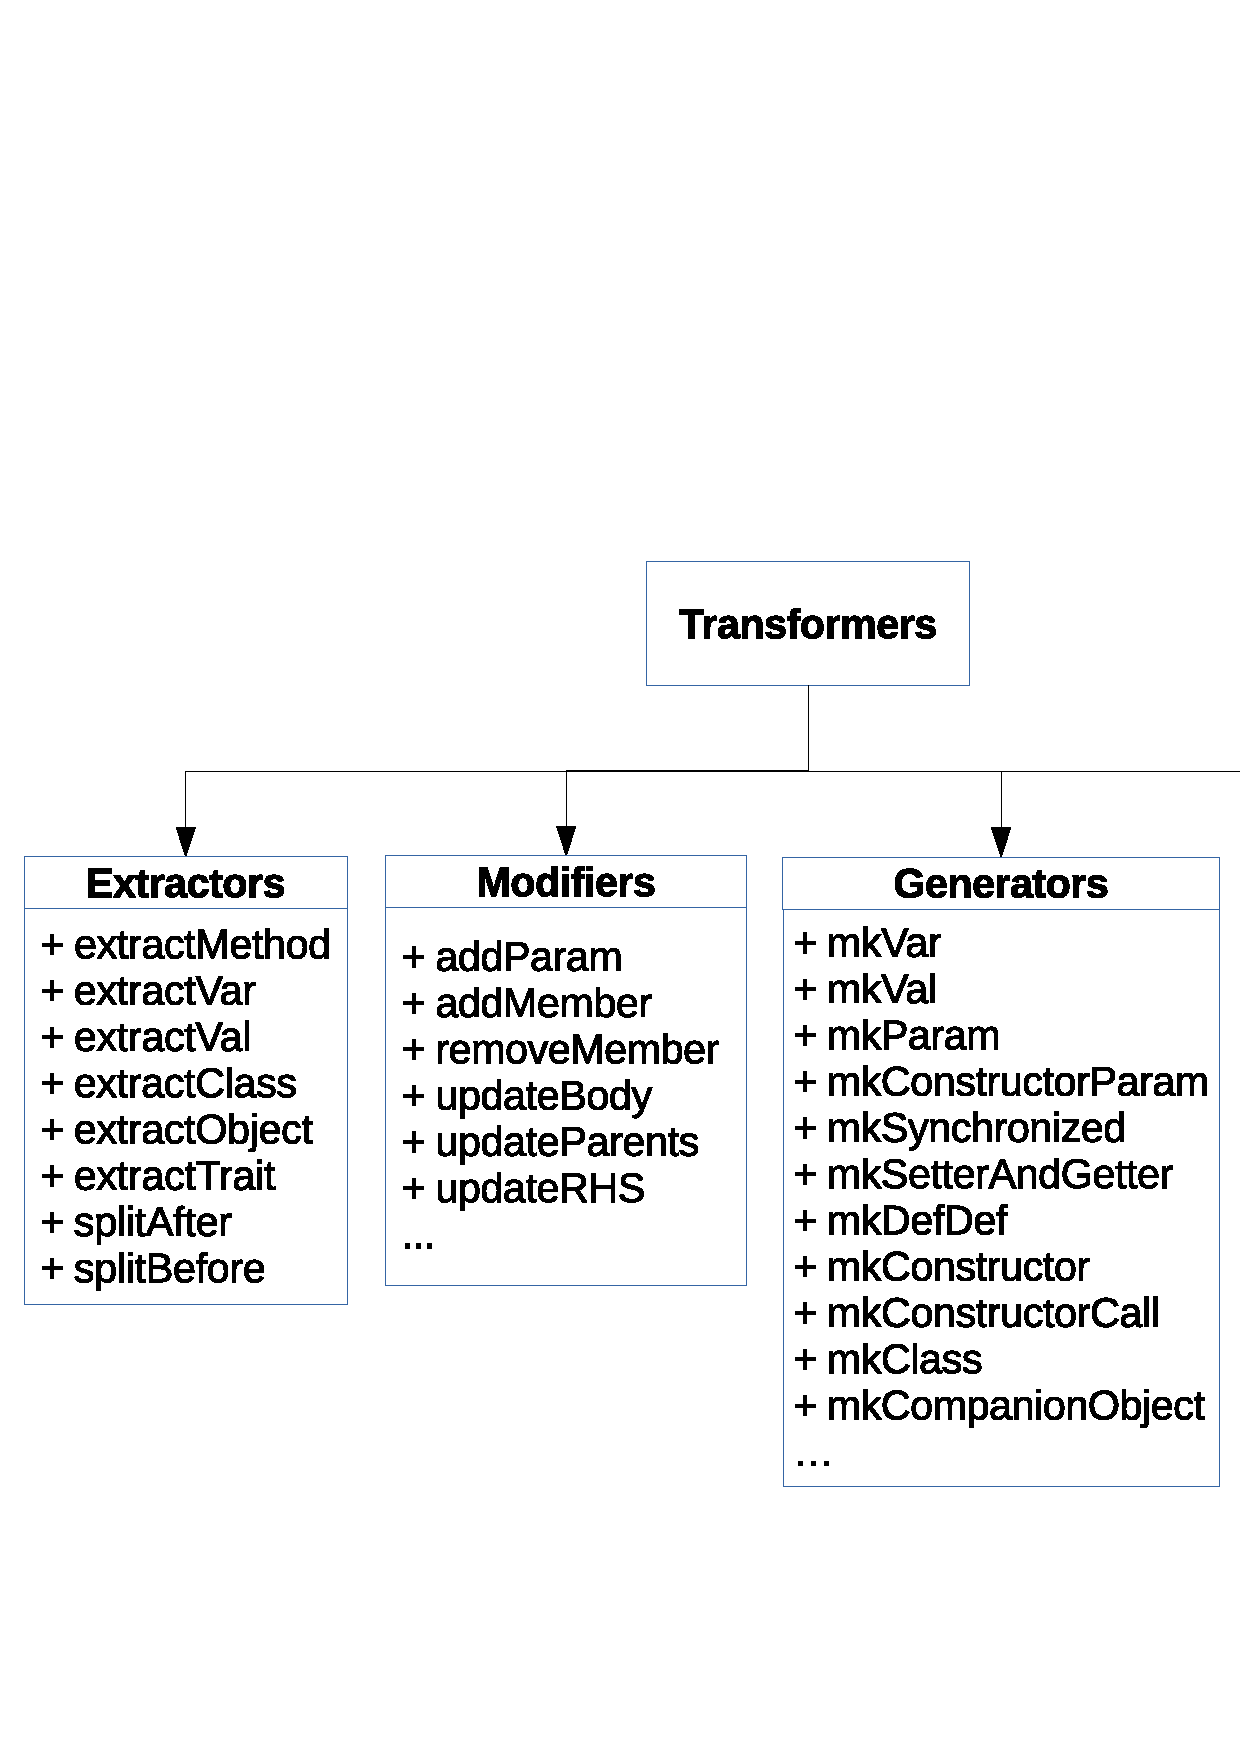
\includegraphics[scale=0.45]{classDiagram}
  \end{center}
  \vspace{-2cm}
  \caption{The high-level design of Lombrello's Library}
  \label{fig:libraryFig}
\end{figure}


\subsection{Tree extractors}

Methods in the \emph{tree extractor} category permit the selection of a
sequence of ASTs to be placed in another, compatible class, object, trait,
method or variable.  Since Scala ASTs are immutable, extractor operations
generate new ASTs and do not affect the original tree to which they are
applied.

Figure~\ref{lst:extractor}(a) shows a code snippet that demonstrates a
refactoring using a pair of tree extractor functions.
Figures~\ref{lst:extractor}(b) and (c) show the effect of applying the
refactoring to a small method.  The extractor function \c{splitAfter} scans the
AST of the body of the original method \c{foo} in
Figure~\ref{lst:extractor}(b).  When \c{splitAfter} finds the first occurrence
of an AST node that satisfies a given predicate and returns the AST before and
include the node and the AST after the node.  In the example, the predicate
matches a call to the \c{splitMe} method, specified using the Scala quasiquotes
library.  Thus \c{splitAfter} returns the AST for the body of \c{foo} up to and
including the call to \c{splitMe}, and another AST for the rest of the body.
  
It is possible to insert either or both of the ASTs returned by \c{splitAfter}
into ASTs.  In Figure~\ref{lst:extractor}(c), \c{suffix} becomes the body of a
new method \c{bar}. This is done by calling \c{extractMethod}, which takes a
list of trees and a new method name as parameters.  The new name must be unique
in its scope, otherwise an exception is thrown.

The \c{extractMethod} operation handles free variables in the given method's
body by adding parameters to the extracted method. That is, all  free variables
in \texttt{suffix} become parameters of \c{bar}.  \c{extractMethod} also
creates the AST of the new method and types it, and generates a call to the
extracted method that can be substituted into the original method, as described
in the next section.  Lombrello also creates a symbol for the new method,
rebinding symbols of the extracted trees to their new owner, and placing them
in the symbol table of the method owner. Without Lombrello, the programmer
would have to perform all these operations manually using the Scala compiler
API.

\begin{figure}[t!]
\begin{lstlisting}
// orig is the original method
// body is the body of orig

// Split body after the call to splitMe(),
val (prefix, suffix) = body.splitAfter((x:Tree) => {
  x == q"splitMe()"
})

// Extract the code after the split into method bar
val (extracted, apply) = extractMethod(
    suffix,     // The body of the extracted method
    "bar"       // the name of the extracted method
    orig.symbol // the symbol of the original method
    ).get

// Replace the extracted code with a call to the new method
orig.updateRHS(Block(prefix, apply))
\end{lstlisting}
      \begin{center}
        (a) 
          A short example of tree extractor and tree modifier utilities
      \end{center}
      \medskip
  \begin{tabular}{cc}
    \begin{minipage}[b]{0.5\textwidth}
\begin{lstlisting}
def foo(a: Int, b: String, 
        c: Int): Int = {

  println(a)
  val d = c
  splitMe()
  println(d)
  a + b.size
} 
\end{lstlisting}
      \begin{center}
        (b) Before applying the refactoring in (a)
      \end{center}
    \end{minipage} &
    \begin{minipage}[b]{0.5\textwidth}
\begin{lstlisting}
def foo(a: Int, b: String, 
        c: Int): Int = {
  println(a)
  val d = c
  splitMe()
  bar(a, b, d)
}
def bar(a: Int, b: Int, 
        d: Int): Int = {
  println(d)
  a + b.size
} 
\end{lstlisting}
      \begin{center}
        (c) After applying the refactoring in (a)
      \end{center}
    \end{minipage}
  \end{tabular}
\caption{A short example of a Lombrello refactoring}
\label{lst:extractExample}
\label{lst:extractor} 
\end{figure}


Other useful Lombrello extractors allow member extraction. It is possible, for
instance, to extract an inner class and make it an outer class (using
\c{extractClass}), to convert a local variable to a field (using \c{extractVar}
or \c{extractVal}), or to move fields or methods across classes.  


Applying Lombrello's extractor functions can sometimes yield malformed trees.
For example, if we add a block extracted from a method that contains a return
statement to a class, the class will not type check. We rely on Scala's type
checker to report such errors to the programmer. 

\subsection{Tree modifiers}

\emph{Tree modifier} utilities change AST nodes, for instance, adding or
removing method parameters (\c{addParam} and \c{removeParam}, respectively),
modifying a class or trait's body (\c{updateBody}, \c{addMember}, and
\c{removeMember}) or its supertypes (\c{updateParents}).  The \c{rename} method
is used to change the name of a class, method, or variable. When a field is
renamed, Lombrello handles renaming its setters and getters as well.  The tree
modifiers also support updating method bodies (\c{updateRHS}).  As an example,
we can modify method \c{foo} from Figure~\ref{lst:extractor}(b) to call the
extracted method, as shown in Figure~\ref{lst:extractor}(c).  We do this with
the call to \c{updateRHS}, as shown in Figure~\ref{lst:extractor}(a). 


\subsection{Tree duplicators}

\emph{Tree duplicators} are mainly used to implement other Lombrello
functionality, but can also be useful when writing plugins. For example, if a
programmer needs to specialize a method, they can duplicate it first, then
remove the specialized parameter from the duplicated tree, and substitute it
with a value, as shown in Figure~\ref{lst:duplicator}.

\begin{figure}[tp]
\begin{lstlisting}
// orig is the method to be specialized
// p is the parameter we want to specialize
// v is the value that we want to specialize p with
val specialized = orig.duplicate("new_name").removeParam(p, v)
\end{lstlisting}
\caption{A simple example showing how a tree duplicator works}
\label{lst:duplicator} 
\end{figure}

Lombrello's \c{duplicate} method differs from the compiler API's \c{duplicate}
method in that it handles the creation of a new symbol for the new tree, and
changes the binding of the node's children's symbols from their original owner
to the duplicate.

The \c{fixOwner} method traverses an AST that has been duplicated and inserted
into the AST at another location. It rebinds symbols in the traversed AST to
change their owner (i.e., containing method, class, etc.) to the symbol at the
new location in the AST.

\subsection{Tree generators}

Lombrello offers various AST generators that are simpler to use than the Scala
compiler API tree generators.  For instance, they handle setting the required
flags that distinguish trees used to represent more than one syntactic
construct (e.g., \c{var} and \c{val}, or class and trait trees). Symbol
creation and binding is also handled for a generated AST, including all its
descendant ASTs.  Lombrello generators facilitate other tasks that require
multiple setup steps, such as surrounding the body of a method with a
synchronization block, creating constructor parameters and constructor calls,
and others. 

\section{Getting More Help}
Lombrello's library is fully documented, you are encouraged to visit the
project's repository and clone it, play with it and understand it.  The
project's repository can be found at
\url{https://github.com/amanjpro/lombrello}. You can generate the Scaladoc by
running

\begin{verbatim}
sbt lombrello/api
\end{verbatim}

You can also take a look at the many plugins that use Lombrello and included in
the project, namely (Avro, Kara, Mina, Atomic Scala and ScalaDyno). You are
welcome to report bugs, suggest improvements and/or contribute to the project.


\section{Software Requirements}
Lombrello should have no problem with Scala 2.11, and in theory it should work 
with newer Scala versions.


\section{Licence}

\begin{verbatim}
Copyright (c) <2013-2014>, Amanj Sherwany <http://www.amanj.me> 
All rights reserved.

Redistribution and use in source and binary forms, with or without
modification, are permitted provided that the following conditions 
are met:
    * Redistributions of source code must retain the above 
      copyright notice, this list of conditions and the 
      following disclaimer.
    * Redistributions in binary form must reproduce the above 
      copyright notice, this list of conditions and the following 
      disclaimer in the documentation and/or other materials provided 
      with the distribution.
    * Neither the name of the <organization> nor the names of its 
      contributors may be used to endorse or promote products
      derived from this software without specific prior written 
      permission.

THIS SOFTWARE IS PROVIDED BY THE COPYRIGHT HOLDERS AND CONTRIBUTORS 
"AS IS" AND ANY EXPRESS OR IMPLIED WARRANTIES, INCLUDING, BUT NOT 
LIMITED TO, THE IMPLIED WARRANTIES OF MERCHANTABILITY AND FITNESS 
FOR A PARTICULAR PURPOSE ARE DISCLAIMED. IN NO EVENT SHALL 
<COPYRIGHT HOLDER> BE LIABLE FOR ANY DIRECT, INDIRECT, INCIDENTAL, 
SPECIAL, EXEMPLARY, OR CONSEQUENTIAL DAMAGES (INCLUDING, BUT NOT 
LIMITED TO, PROCUREMENT OF SUBSTITUTE GOODS OR SERVICES; LOSS OF USE, 
DATA, OR PROFITS; OR BUSINESS INTERRUPTION) HOWEVER CAUSED AND
ON ANY THEORY OF LIABILITY, WHETHER IN CONTRACT, STRICT LIABILITY, 
OR TORT (INCLUDING NEGLIGENCE OR OTHERWISE) ARISING IN ANY WAY OUT 
OF THE USE OF THIS SOFTWARE, EVEN IF ADVISED OF THE POSSIBILITY 
OF SUCH DAMAGE.

\end{verbatim}



\end{document}
